\newpage

\subsection{Сравнительный анализ результатов моделирования}

Сравнение результатов аналитического и имитационного моделирования приведено ниже в таблице~\ref{table:result_compr}.

\begin{table}[h]
\caption{Сравнение аналитического и имитационного моделирования}
\label{table:result_compr}
\centering
 \begin{tabular}{c}
 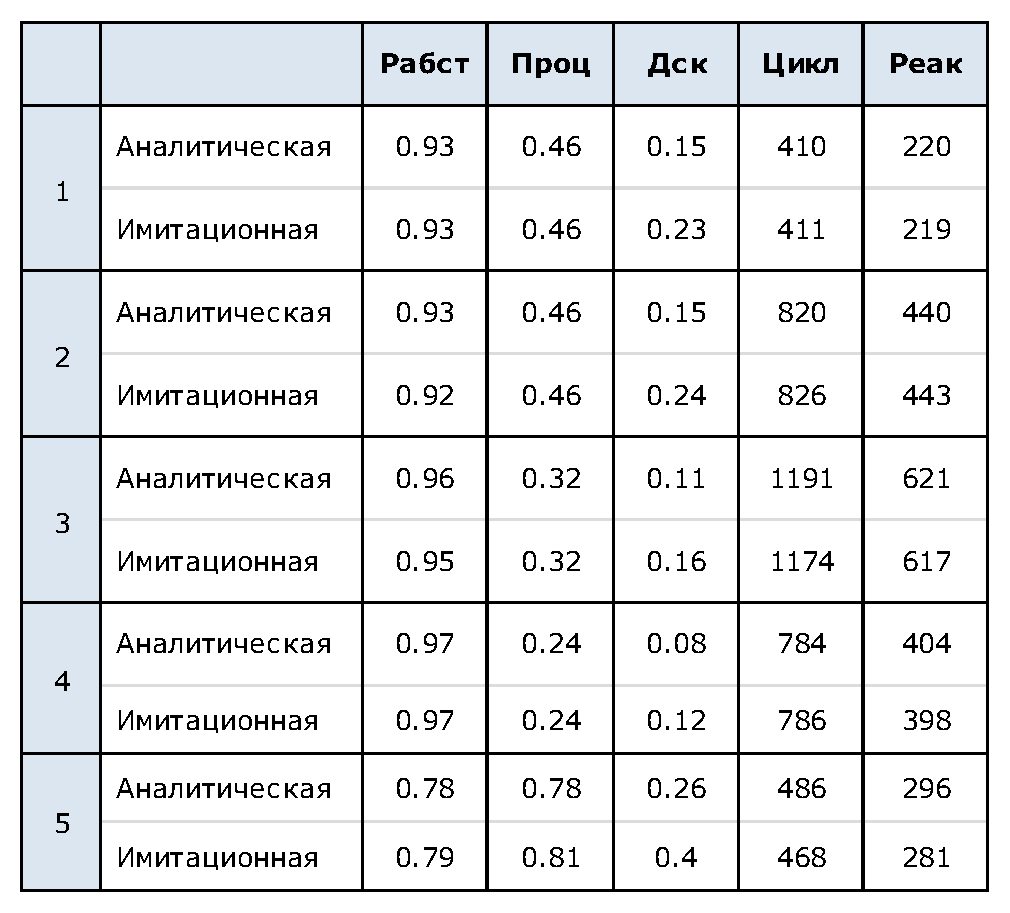
\includegraphics[width=0.7\linewidth]{pics/pic12_1_result_compr.eps}
 \end{tabular}
\end{table}

Сравнительный анализ приведенных результатов показывает, что различие между результатами аналитического и имитационного моделирования составляет не более 10\%. Это вполне приемлемый для инженерных расчётов результаанализ приведенных результатов показывает, что различие между результатами аналитического и имитационного моделирования составляет не более 10\%. Это вполне приемлемый для инженерных расчётов результат.\par\bigskip

Разница в значениях между аналитическим и имитационным моделированием объясняется следующими причинами:
\begin{itemize}
\item при аналитическом моделировании методом фонового потока использовали приближённый итерационный алгоритм нахождения значений выходных характеристик рассматриваемой системы;
\item при имитационном моделировании на языке GPSS задавали ограниченное время моделирования и использовали приближенную экспоненциальную функцию распределения времени обслуживания, которую задавали по точкам.
\end{itemize}